% Chapter 1

k\chapter{A Language of Polynomials} % Main chapter title

\label{Chapter1} % For referencing the chapter elsewhere, use \ref{Chapter1} 

%----------------------------------------------------------------------------------------

% Define some commands to keep the formatting separated from the content 
\newcommand{\keyword}[1]{\textbf{#1}}
\newcommand{\tabhead}[1]{\textbf{#1}}
\newcommand{\code}[1]{\texttt{#1}}
\newcommand{\file}[1]{\texttt{\bfseries#1}}
\newcommand{\option}[1]{\texttt{\itshape#1}}

%----------------------------------------------------------------------------------------

\section{Introduction}
This paper is on the re-framing of the one way function to a matrix multiplication problem - that of multiplying two $3 \times 3$ matrices to form a $6 \times 6$ matrix under a locally concatenative property.

%----------------------------------------------------------------------------------------

\section{Foundations}

There exists a language such that it decides each monomial in the polynomial. In other words, there exists a set of deciders for each monomial in the polynomial where it decides if y is in the monomial. A decider in this term is not of the definition found originally in textbooks but one that is redefined in the below definition.

$\newline$

Given a polynomial

$p(x) = ax^2 + bx + c$

$p(x) = 3x^2 + 4x + 5$

$p(2) = 3(2)^2 + 4(2) + 5$

$p(2) = 12 + 8 + 5$

$\newline$

Let the decider be defined as the following:

$\\ $

Decider is a function $Decider<c \times x^{degree}> \equiv c \times x^{degree} = y$

such that
$x_1 \times x_2 \times ... \times x_n\ $ where n is equal to degree + constant is tested to be equivalent to y
and $x_1$ is the start
and $x\ degree\ times$ is the finish
then loop around $x_1 to x\ degree\ times$ until it stops

For each state, $x_i$, i such that it is between 1 to n, $x_i$ contains a subgroup of size n and for each subgroup, $s_i$, there exists another subgroup and so on and so forth such that there are n layers starting from $x_i$ to 1. This is the same as saying that it is a rational expression.

$\newline$

A rational expression is a expression that satisfies the following.
$\\ $

$A_n = A_{n-1} \cup  {\left\{  E^* | E \in \mathcal{E}_{n-1}, (E,1)=0 \right\}}$

$\newline$

$\textbf{Examples}$

Decider for $ax^2$ is $Decider(3,2,2) = 3(2)^2 \equiv 12$

Decider for $bx$ is $Decider(4,2,1) = 4(2)^1 \equiv 8$

Decider for $c$ is $Decider(1,2,1) = 5(2)^0 \equiv 5$

$\\ $

\begin{figure}[h]
  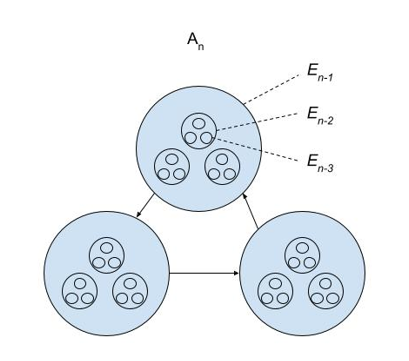
\includegraphics[width=\linewidth]{0101DeciderX3.png}
  \caption{Decider X to the 3.}
  \label{fig:0101DeciderX3}
\end{figure}
Figure \ref{fig:0101DeciderX3} shows a monomial decider, $Decider<x^n>$ with that represents $x^3$.

$\\ $

It follows that each state $E \in s_{n-1}$ forms a subgroup.

$\\ $

A rational function is defined as the following: 

K[x] and K[[x]]. Let K[[x]] describe a set of monomial deciders. S is an element of K[[x]] meaning S is a monomial decider.

S = $\sum_{n\geq 0}{a_n x^n}$

$\\ $

$\textbf{Theorem}$: A Decider is the equivalent to a cyclic automata

$\\ $

$\textit{Proof}$: Remove the lowest level state, $S_1$ from the bottom then continue removing $S_i$ from i = 2 to n-1 until you get only the states that are at $X_n$.

$\\ $

Remove the top state down from the $S_{n-1}$ for each layer $S_{n-1}$ to $S_(n-n-1)$. This preserves the start and finish state for the layer $x_{n}$. This is a cyclic automaton.

$\\ $

\begin{figure}[h]
  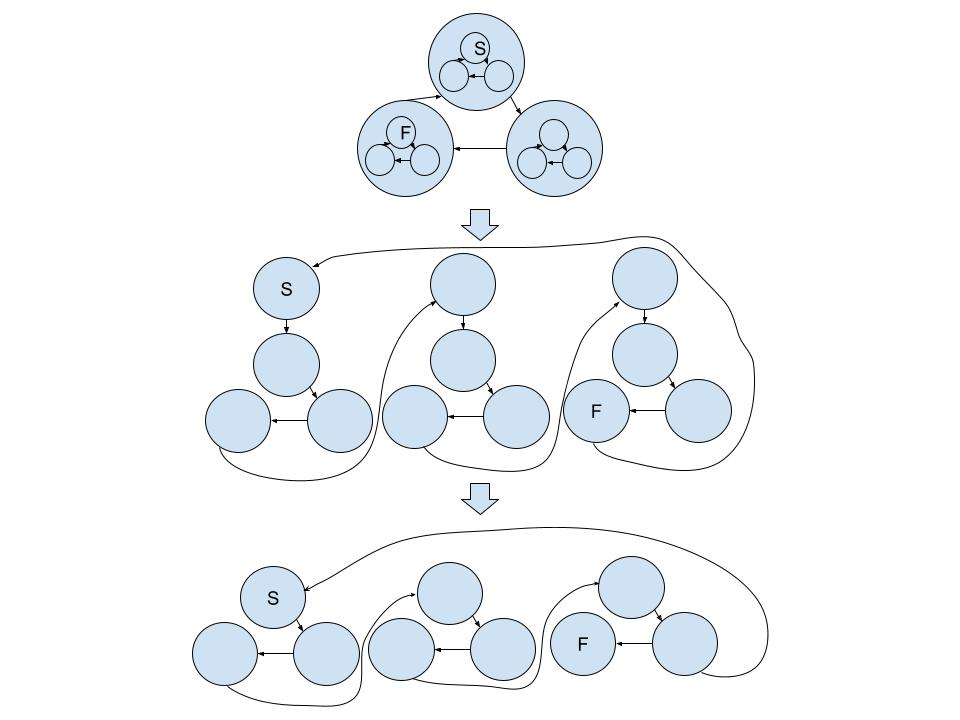
\includegraphics[width=\linewidth]{0102theorem.jpg}
  \caption{Top down removal for equivalence of decider and cyclic automata.}
  \label{fig:0102theorem}
\end{figure}
Figure \ref{fig:0102theorem} shows how the intuition for removing the state top down.

\section{Monomial of One Degree}

Given the definition of a decider:
%Decider is a function Decider(constant,x,degree)≡constant∗xdegree=y

A decider of at least one degree

$Decider(3,x,4) \equiv 3x^4 = y$

Contains $Decider(3,x,3) \equiv 3x^3 = y$

Contains $Decider(3,x,2) \equiv 3x^2 = y$

Contains $Decider(3,x,1) \equiv 3x^1 = y$

Contains $Decider(3,x,0) \equiv 3x^0 = y$

Hence it can be generalized to:

$Decider(constant,degree,x)$ contains the sequence set 

$Decider constant,degree,x ,Decider constant,degree 1,x,...,Decider constant,0,x $

$\{start,...,finish\}$

\section{Addition}

Given the first example:

p(x)=3x2+4x+5

p(2)=3(2)2+4(2)+5

p(2)=12+8+5


m2=Decider(3,x,2)=3x2

m1=Decider(4,x,1)=4x

m0=Decider(5,x,0)=5


Generalized to mx where x is the degree

Given polynomial functions, p1 and p2, they are commutative

p1(x)=ma+...+m0

p2(x)=nb+...+n0

p1(x)+p2(x)=ma+m[x+1]+nb+n[y+1]+...+(mx+ny)+...+(m0+n0) where x=y

Decider(cx,x,dx)

+Decider(cy,x,dy)=Decider(cx+cy,x,dx)=Deciders(cx+cy,x,dy)= dx=dy

\section{Product}

Given two monomials in the language, a and b, the product of a and b is also in the language.

Given Decider(cx,x,dx) and Decider(cy,x,dy) is in language L

Show that the product Decider(cx+cy,x,dx$\times $dy) is in L

Decider(cx,x,dx)$\times $Decider(cy,x,dy)

=cx$\times $xdx$\times $cy$\times $xdy

=cx$\times $xdx+dy

=(cx+cy)$\times $xdx+dy is in L

=Decider(cx+cy,x,dx+dy)

\section{Problem with Matrices}


Given a polynomial p of x, show that the monomial deciders represented in the language can't be contained in a finite matrix after a set number, n, such that x$n$.

axa $\times $ bxb = nxn such that a $\neq $ b and a,b<n

\section{Multivariable Polynomials}

A monomial with more than one variable can be treated the same way as handling single variables at different degrees.

Decider(c,xyz,d) = c(xyz)d = Decider(c,x,d)$\times $Decider(c,y,d)$\times $Decider(c,z,d) where c is some constant
Decider(c,x,d1)$\times $Decider(c,y,d2)$\times $Decider(c,z,d3) = cxd1$\times $yd2$\times $zd3 where c is some constant

Given f(x,y)=3xy2

set x=2,y=3

f(2,3)=3(2)(3)2

f(2,3)=27

\section{Generalized Monomial Deciders}

A monomial decider can be represented in a more general graphic

6x6=Decider 6,x,6 =6$\times $ xstart,x2,x3,x4,x5,xfinish 
 x6=Decider 1,x,6 =1$\times $ xstart,x2,x3,x4,x5,xfinish 


In both these examples, xstart is x1 and xfinish is x6.


\section{Concentric Monomial Deciders}

Given a polynomial, p x, with a monomial decider represented as ax n in p x and n in N and a = 1 such that p x = x n, there is special property for these monomial deciders that can be illustrated below.

Decider 1,x,4 = x = xi such that i is in start,2,3,finish and xi contains xi minus 1 where i 1
 Decider 1,x,2 = x2 = xi such that i is in start,finish and xi contains xi minus 1 where i 1
 In both these examples, xi is a state in the monomial decider.
Each state in a one constant monomial decider have a property of being concentric. This means that a state can be defined as, x2 =
 x1,x0 so going from x1 to x0 then going to the next state x3 or looping back to x1.
 
\section{Constants}

Given a constant, c, of p or better described in the example: f(x) = 5. Constants are seen as linear directed acyclic graphs.

f(x) = 5

$Decider(5,x,0) \equiv 5 \equiv {start,2,3,4,finish}$

There is no state in the decider where it loops back to the start. In other words, there is no x that represents a monomial in a constant.

\section{Division}

Division of monomial deciders


$x^5 / x = x^4 \equiv Decider(1,x,5)/Decider(1,x,1) ~ Decider(1,x,4)$
$x^5 / x^2 = x^3 \equiv Decider(1,x,5)/Decider(1,x,2) ~ Decider(1,x,3)$
$x^5 / x^3 = x^2 \equiv Decider(1,x,5)/Decider(1,x,3) ~ Decider(1,x,2)$
$x^5 / x^4 = x^1 \equiv Decider(1,x,5)/Decider(1,x,4) ~ Decider(1,x,1)$
$x^5 / x^5 = 1 \equiv Decider(1,x,5)/Decider(1,x,5) ~ Decider(1,x,0)$

~ here is represented as a special kind of equivalence that we will get to later.

$Decider(1,x,5)/Decider(1,x,1) \equiv
 {sequence of permutations of {xi,xj} such that the count of i is 4 and j is 1}$
$Decider(1,x,5)/Decider(1,x,2) \equiv
 {sequence of permutations of {xi,xj} such that the count of i is 3 and j is 2}$
$Decider(1,x,5)/Decider(1,x,3) \equiv
 {sequence of permutations of {xi,xj} such that the count of i is 2 and j is 3}$
$Decider(1,x,5)/Decider(1,x,4) \equiv
 {sequence of permutations of {xi,xj} such that the count of i is 1 and j is 4}$
$Decider(1,x,5)/Decider(1,x,5) \equiv
 {sequence of permutations of {xi,xj} such that the count of i is 0 and j is 5} Here, xi \neq
 xj, meaning xi is of a different representation than xj$

\section{Multiple Divisions}

Given multiple operations of division, this forms an interesting space.
x5/x2/x=x5/x)/x2

Decider 1,x,5 /Decider 1,x,2 /Decider 1,x,1 =Decider 1,x,5 /Decider 1,x,1 /Decider 1,x,2
 iff ignoring order of operations
 
\section{Equivalence}

Decider 1,x,6 /Decider 1,x,1 /Decider 1,x,1 ~Decider 1,x,6 /Decider 1,x,2
  iff the order of operations is next to each other

Determining if y is in f x is easy if we are given any monomial decider in the set of the language of polynomials and their representations has the possibility to give different representations if we consider them as representations of the function f x.

Decider 1,x,6 /Decider 1,x,1 /Decider 1,x,1 =sequence of permutations of xi,xj,xk such that the count of i is 4 and j is 1 and k 1


Decider 1,x,6 /Decider 1,x,2 =sequence of permutations of xi,xj such that the count of i is 4 and i is 2


Theorem of Equivalence
Decider 1,x,6 /Decider 1,x,1 /Decider 1,x,1 =Decider 1,x,6 /Decider 1,x,2 such that there is some xsuch that the monomial represented by both deciders exists where f x =y

\section{Theorem of Equivalence}

$
Decider(1,x,6)/Decider(1,x,1)/Decider(1,x,1) \\
    \equiv Decider(1,x,6)/Decider(1,x,2) \\
        such\ that\ there\ is\ some\ x \\
        such\ that\ the\ monomial\ represented\ by\ both\ deciders\ exists\ where\ f(x) \equiv y
$ 

\section{Reversing}

$Decider(1,x,6)/Decider(1,x,1)/Decider(1,x,1) \equiv {sequence\ of\ permutations\ of\ {xi,xj,xk}\ such\ that\ the\ count\ of\ i\ is\ 4\ and\ j\ is\ 1\ and\ k\ 1}$

$Decider(1,x,6)/Decider(1,x,2) \equiv {sequence\ of\ permutations\ of\ {xi,xj}\ such\ that\ the\ count\ of\ i\ is\ 4\ and\ i\ is\ 2}$

Is shown that by the permutation of the order of operations that $Decider(1,x,6)/Decider(1,x,1)/Decider(1,x,1)$ is not the same set as $Decider(1,x,6)/Decider(1,x,2)$

Theorem of Reversing

Given two deciders x,y in a decider of m(x), x != y iff sequence of all the states are not equivalent, representation-wise, from start to finish or it doesn't represent the same order of operations of the deciders being represented

\section{Corollary of Reversing}

A little more on the theorem of reversing
Given a starting point, the paths a monomial decider takes to decide if y is in f x is inherently unique to each representation. Start at the circle, S, and end at the circle, F. If the circle is white, it is 0. If it is blue, it is 1. As an example let's traverse some of the representations of x 4.

Corollary
Given a decider, d, in Decider of m x then there is path, p, that exists for d such that p = Path d = s1,s2,...,si,...,sn where i is count of the states in the decider of m x.

Example:
Choose some x such that it is in Path Decider 1,x,6/Decider1,x,2 where p = 001111

\section{Godel's Theorem}

We see that there exists two statements from these theorems

1. x = x from a theorem of equivalence
2. x != x from a theorem of reversal


Example:
Given some d1,d2,d3,...,infinity in deciders of m x
1. d1 = d2 = d3 = ... = infinity
2. d1 != d2 != d3 = ... != infinity

The different representations of a monomial through the language of monomial deciders will give us undecidability. This means we can come up with many formal definitions of the mnomial decider and it will not be able to solve the problem of finding a specific representation of a monomial decider without having to guess or apply some sort of probability to it. Relating to the real line, given a real line a,b a $\leq$ b, there is infinite choices between a and b because we canjust make the number smaller. As long as b  a $\geq $ 0, there requires some sort of probability of choosing some specific number that is between a and b.

\section{Reframing The One Way Function}

A probability exists to find a certain monomial decider in the set of it's variations. A/B = Probability where A is the monomial decider we want and B is the number of all the variations.

Example:
d1,d2,...,d6 in deciders 1,x,6 ,D, such that di are all distinct
Choose one of the deciders in D through probability
Probability of choosing d in D is 1/6 so 0.16666667
We'll call this picking a function and every time we call this function, the probability is mulltiplied such that it is n k. As an example, if we call the picking function twice using the example above, we have 1/6 1/6 = 1/36 = 6 2.

This is formally known as the one way function.

\section{Theorem of Infiniteness}

Given that, if we can show for any language it abides a theorem of equivalence and a theorem of reversal and they both have infinite representations, we know that we need some sort of probability to choose a specific representation of a monomial decider. We'll call this a theorem of infiniteness because if we can show that some language is infinite, it will require some sort of guess to pick something unique out of all the things it represents, generates, or describes. In other words, you can't map infinity to infinity directly for you must map infinity to something discrete and something discrete to infinity.

Theorem
A mapping must be from infinity to discrete representation to discrete representation to infinity.

Given any representation of infinity,
Suppose a mapping infinity to infinity exists.
Then this map is equivalent to infinity because 
infinity contains this map.
Here, infinity is represented as $\ast. \ast contains \ast -> \ast.$

Intuition

Given Decider c,x,d and d is infinity,
Decider c,x,d contains Decider c,x,d 1
d 1 is then infinity too.


\subsection{References}

The \code{biblatex} package is used to format the bibliography and inserts references such as this one \parencite{Reference1}. The options used in the \file{main.tex} file mean that the in-text citations of references are formatted with the author(s) listed with the date of the publication. Multiple references are separated by semicolons (e.g. \parencite{Reference2, Reference1}) and references with more than three authors only show the first author with \emph{et al.} indicating there are more authors (e.g. \parencite{Reference3}). This is done automatically for you. To see how you use references, have a look at the \file{Chapter1.tex} source file. Many reference managers allow you to simply drag the reference into the document as you type.

Scientific references should come \emph{before} the punctuation mark if there is one (such as a comma or period). The same goes for footnotes\footnote{Such as this footnote, here down at the bottom of the page.}. You can change this but the most important thing is to keep the convention consistent throughout the thesis. Footnotes themselves should be full, descriptive sentences (beginning with a capital letter and ending with a full stop). The APA6 states: \enquote{Footnote numbers should be superscripted, [...], following any punctuation mark except a dash.} The Chicago manual of style states: \enquote{A note number should be placed at the end of a sentence or clause. The number follows any punctuation mark except the dash, which it precedes. It follows a closing parenthesis.}

The bibliography is typeset with references listed in alphabetical order by the first author's last name. This is similar to the APA referencing style. To see how \LaTeX{} typesets the bibliography, have a look at the very end of this document (or just click on the reference number links in in-text citations).

\subsubsection{A Note on bibtex}

The bibtex backend used in the template by default does not correctly handle unicode character encoding (i.e. "international" characters). You may see a warning about this in the compilation log and, if your references contain unicode characters, they may not show up correctly or at all. The solution to this is to use the biber backend instead of the outdated bibtex backend. This is done by finding this in \file{main.tex}: \option{backend=bibtex} and changing it to \option{backend=biber}. You will then need to delete all auxiliary BibTeX files and navigate to the template directory in your terminal (command prompt). Once there, simply type \code{biber main} and biber will compile your bibliography. You can then compile \file{main.tex} as normal and your bibliography will be updated. An alternative is to set up your LaTeX editor to compile with biber instead of bibtex, see \href{http://tex.stackexchange.com/questions/154751/biblatex-with-biber-configuring-my-editor-to-avoid-undefined-citations/}{here} for how to do this for various editors.
